
\documentclass{standalone}
\usepackage[T1]{fontenc}\usepackage{tikz}
\usepackage{amsmath, amsfonts}
\usetikzlibrary{arrows.meta}
\begin{document}
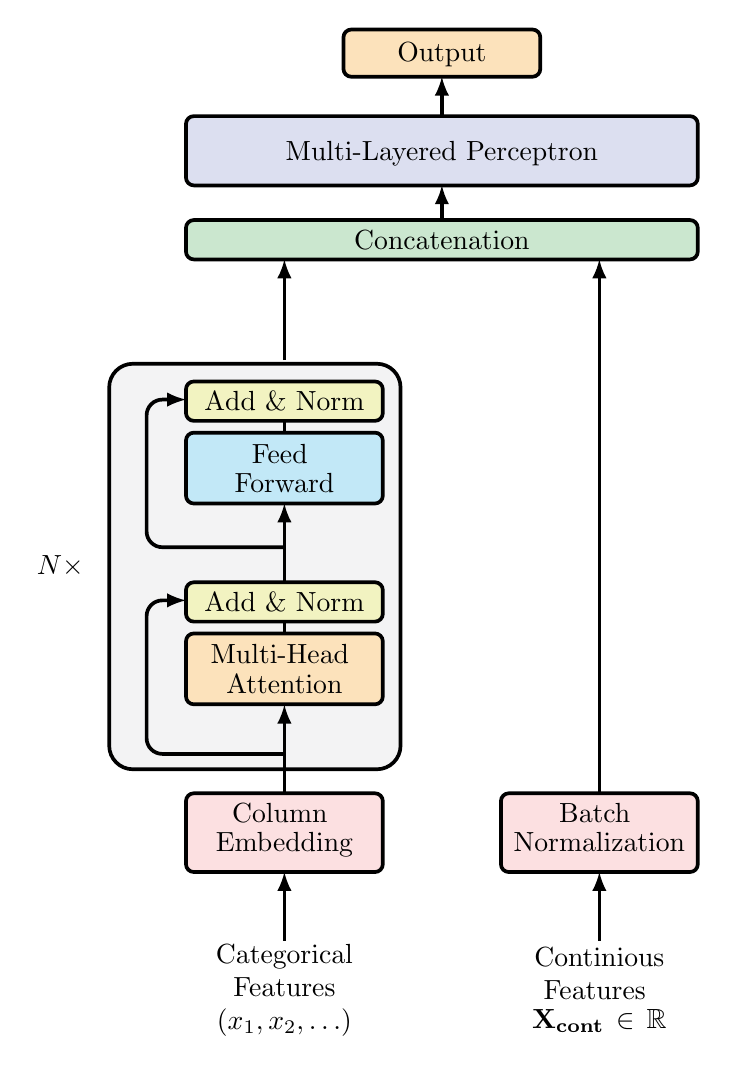
\begin{tikzpicture}
\definecolor{emb_color}{RGB}{252,224,225}
\definecolor{multi_head_attention_color}{RGB}{252,226,187}
\definecolor{add_norm_color}{RGB}{242,243,193}
\definecolor{ff_color}{RGB}{194,232,247}
\definecolor{softmax_color}{RGB}{203,231,207}
\definecolor{linear_color}{RGB}{220,223,240}
\definecolor{gray_bbox_color}{RGB}{243,243,244}


\draw[fill=gray_bbox_color, line width=0.046875cm, rounded corners=0.300000cm] (-0.975000, 8.455000) -- (2.725000, 8.455000) -- (2.725000, 3.305000) -- (-0.975000, 3.305000) -- cycle;


\draw[line width=0.046875cm, fill=multi_head_attention_color, rounded corners=0.100000cm] (2.0, 12.70000) -- (4.500000, 12.7) -- (4.500000, 12.10000) -- (2.0, 12.1) -- cycle;
\node[text width=2.500000cm, anchor=south, align=center] at (3.250000,12.10000) {Output};

\draw[line width=0.046875cm, fill=linear_color, rounded corners=0.100000cm] (0.0, 11.60000) -- (6.500000, 11.6) -- (6.500000, 10.720000) -- (0.000000, 10.720000) -- cycle;
\node[text width=5.00000cm,  align=center] at (3.25,11.130000) {Multi-Layered Perceptron};

\draw[line width=0.046875cm, fill=softmax_color, rounded corners=0.100000cm] (0.0, 10.280000) -- (6.500000, 10.28) -- (6.500000, 9.780000) -- (0.000000, 9.780000) -- cycle;
\node[text width=5.00000cm,  align=center] at (3.25,10.030000) {Concatenation};

\draw[line width=0.046875cm, fill=emb_color, rounded corners=0.100000cm] (0.000000, 3.00000) -- (2.500000, 3.00000) -- (2.500000, 2.0000) -- (0.000000, 2.000) -- cycle;
\node[text width=2.500000cm, anchor=north, align=center] at (1.250000,3.00000) {Column \vspace{-0.05cm} \linebreak Embedding};


\draw[line width=0.046875cm, fill=emb_color, rounded corners=0.100000cm] (4.000000, 3.00000) -- (6.500000, 3.00000) -- (6.500000, 2.0000) -- (4.000000, 2.000) -- cycle;
\node[text width=2.500000cm, anchor=north, align=center] at (5.250000,3.00000) {Batch \vspace{-0.05cm} \linebreak Normalization};


\node[text width=2.500000cm, align=center] at (1.250000,0.50000) {Categorical Features \linebreak $(x_1, x_2, \hdots)$};
\node[text width=2.500000cm, align=center] at (5.250000,0.5) {Continious Features \vspace{-0.05cm} \linebreak $\bf{X}_{cont} \in \mathbb{R}$};


\draw[line width=0.046875cm, -latex] (1.250000, 1.125) -- (1.250000, 2.0);
\draw[line width=0.046875cm, -latex] (1.250000, 3.0) -- (1.250000, 4.125);
\draw[line width=0.046875cm, -latex] (1.250000, 8.5) -- (1.250000, 9.78);

\draw[line width=0.046875cm, -latex] (5.250000, 1.125) -- (5.250000, 2.0);
\draw[line width=0.046875cm, -latex] (5.250000, 3.0) -- (5.250000, 9.780);

\draw[line width=0.046875cm, -latex] (3.25, 10.28) -- (3.25, 10.72);
\draw[line width=0.046875cm, -latex] (3.25, 11.6) -- (3.25, 12.1);

\draw[line width=0.046875cm, fill=add_norm_color, rounded corners=0.100000cm] (0.000000, 5.680000) -- (2.500000, 5.680000) -- (2.500000, 5.180000) -- (0.000000, 5.180000) -- cycle;
\node[text width=2.500000cm, align=center] at (1.250000,5.430000) {Add \& Norm};

\draw[line width=0.046875cm, fill=multi_head_attention_color, rounded corners=0.100000cm] (0.000000, 5.030000) -- (2.500000, 5.030000) -- (2.500000, 4.130000) -- (0.000000, 4.130000) -- cycle;
\node[text width=2.500000cm, align=center] at (1.250000,4.580000) {Multi-Head \vspace{-0.05cm} \linebreak Attention};

\draw[line width=0.046875cm, fill=ff_color, rounded corners=0.100000cm] (0.000000, 7.580000) -- (2.500000, 7.580000) -- (2.500000, 6.680000) -- (0.000000, 6.680000) -- cycle;
\node[text width=2.500000cm, align=center] at (1.250000,7.130000) {Feed \vspace{-0.05cm} \linebreak Forward};

\draw[line width=0.046875cm, fill=add_norm_color, rounded corners=0.100000cm] (0.000000, 8.230000) -- (2.500000, 8.230000) -- (2.500000, 7.730000) -- (0.000000, 7.730000) -- cycle;
\node[text width=2.500000cm, align=center] at (1.250000,7.980000) {Add \& Norm};



\draw[line width=0.046875cm] (1.250000, 5.030000) -- (1.250000, 5.180000);
\draw[line width=0.046875cm] (1.250000, 7.580000) -- (1.250000, 7.73);
\draw[line width=0.046875cm, -latex] (1.250000, 5.68) -- (1.250000, 6.68);

\draw[-latex, line width=0.046875cm, rounded corners=0.200000cm] (1.25, 3.5) -- (-0.50000, 3.5) -- (-0.5, 5.45) -- (0, 5.45);
\draw[-latex, line width=0.046875cm, rounded corners=0.200000cm] (1.25, 6.125) -- (-0.50000, 6.125) -- (-0.5, 8.0) -- (0, 8.0);

\node[anchor=east] at (-1.175000,5.880000) {$N\times$};

\end{tikzpicture}
\end{document}